%For an example of a full page figure, see Fig.~\ref{fig:myFullPageFigure}.
\graphicspath{{figures/Oculus/}}

\chapter{The Oculus Vision System}
\section{Motivation}
There is great interest in development of complex vision systems for robotic vision applications. Such research has strict requirements; these systems must operate in real-time, using input from multiple sources, and typically consist of multiple algorithms which work in concert to produce useful output with minimal delay. Consequently, the architecture which binds algorithms and input sources together has become an increasingly important factor. In this Appendix we shall present a vision architecture we developed over the course of the thesis work which uses modular plugins, a novel buffering scheme, and GPU memory optimizations to allow real-time performance of an online vision system, even with complex pipelines and algorithms developed by independent researchers.

A primary concern when developing such complex vision systems lies in how to properly integrate algorithms developed by different researchers, often from multiple institutions. Typically, computer vision researchers develop solutions tailor-made for their particular problem, without concern over the difficulties involved in integrating their particular algorithm into a large system. To ease this integration process, we provided a plugin interface. The plugin system allows independently developed algorithms to communicate with the architecture's central memory management system, interact with the GUI, define their own unique data types, and integrate into systems with plugins developed by other researchers.

Another motivation for developing a vision architecture is the desire to enable the use of complex algorithmic layouts in an online system. In particular, interest in creating loops that allow high level algorithms (i.e. which come late in the pipeline) to feedback and improve the output of low level vision methods. Traditional online vision pipeline architectures cannot accommodate such loops in an adequate way, as at any given moment each portion of the pipeline is processing data from different instants in time. 

Existent vision system architectures also do not support the use of GPUs in a fully integrated way, leading to inefficient use of the device and communication with device memory. The presented method incorporates specially designed GPU data-containers to ensure optimal PCI-bus use through a pre-caching scheme and concurrent memory transfers. In addition to these, extensibility is ensured through an interface which allows user-defined data-container handling, allowing plugin developers to explicitly define how the memory manager shares data between the host and device. In this Appendix we will present an overview of our system, describe a typical system configuration used for robotics, and then give performance figures from a demonstration setup.

%\section{Related Work}
%The most widely used vision software in the field is the OpenCV library, thanks to its permissive license, active development, and large gamut of algorithms. While useful in accelerating the creation of algorithms, OpenCV lacks many of the tools needed for construction of a complete vision system \cite{CVFrameworks}. In particular, OpenCV has limited visualization support, lacks a framework for constructing complex streaming pipelines, and has only recently begun adding GPU support. 
%There are a few existing open-source projects centered around computer vision system architecture, such as iceWing \cite{Icewing} and Imalab \cite{Imalab}. These systems bear some similarities to ours, in that they are sophisticated vision development environments, featuring modularity, efficient visualization, and simple control of algorithm parameters. While a step forward, these projects lack two core features required for our work; support of feedback loops and integrated use of the GPU as a coprocessor. 
%In addition to the open-source projects, there are a few commercial solutions available. Foremost among these is MATLAB, which uses a high-level scripting language to allow for rapid development. Unfortunately, its restrictive and expensive licensing can make it difficult to develop algorithms in distributed locations; every developer must have not only a MATLAB license, but also licenses for the multiple toolboxes required. Additionally, since MATLAB (and it's open source equivalent Octave) development is not in C/C++, creation of novel GPU algorithms using a language such as CUDA is difficult. Other commerical solutions, such as HALCON \cite{HALCON} or BLOX \cite{BLOX} also suffer from their restrictive licensing, making them not well suited for research. None of these solutions permit feedback loops in a real-time online vision system.

%%%%%%%%%%%%%%%%%%%%%%%%%%%%%%%%%%%%%%%%%%%%%%%%%%%%%%%%%%%%%%%%%%%%%%
%%%%%% SYSTEM ARCHITECTURE %%%%%%%%%%%%%%%%
%%%%%%%%%%%%%%%%%%%%%%%%%%%%%%%%%%%%%%%%%%%%%%%%%%%%%%%%%%%%%%%%%%%%%%
\section{System Architecture}

Our vision system is a plugin shell which provides an easy-to-use API for interacting with the GUI, memory management system, and visualization components. In order to ensure expandability, such a system must provide straightforward communication and interaction between plugins created independently, while employing strong-typing checks to ensure only valid plugins may be inter-connected. In addition, it must ensure that plugins have the flexibility to define their own methods for visualization. Finally, the system must ensure that each plugin is self-contained, and executes within its own thread (or threads). This is especially important for fast execution on modern processors, where the number of cores can match, or even exceed, the number of plugins one is running. 

In the next subsections, we shall describe how our architecture accomplishes these goals while requiring as little computational and communication overhead as possible. Small overhead is especially important in the case of real time video processing, where relatively large images must be processed at fast frame rates. 

\subsection{Execution Flow}
At its core, the architecture provides a shell which consists of a GUI for loading plugins and visualizing data, a system for storing plugin output to file, and a buffering/memory-management system for handling data. This functionality is contained in the \emph{Main Thread} and \emph{Memory Manager Thread} shown in Figure~\ref{fig:SystemArchitecture}. Users build their system by adding plugins, configuring their options via the GUI, and then connecting the plugins to each-other. The user can also save/load a fully configured system as an XML file. Once a vision system has been built, the user can control execution using the frame rate module, which controls the firing rate of the system clock. 

As the whole system runs asynchronously in independent threads, the clock trigger acts as the initial starting point for each frame. This means that any source plugins, such as a stereo camera rig or a video file reader plugin, must connect to the frame rate module. As a trigger arrives at each plugin, a triggering signal is sent to the memory manager, telling it to generate a \emph{DataContainer} for the plugin's output. The plugin is then triggered, causing it to execute its processing functionality and generate output, which it stores in the location assigned to it by the memory manager. The plugin then generates another triggering signal, which is connected to both the memory manager and whatever ensuing plugins use the output as their input. When a plugin has multiple inputs, it will loop inside its execution thread, waiting until all inputs for a frame have arrived before executing. This is accomplished by each thread having its own input queue map; it is important to note though, that these queues 
contain no actual data (and thus minimal overhead), and merely serve as a message passing system. The signaling and triggering system employs the open-source Qt signal \& slot architecture. In particular, the system makes use of Qt's ability to queue signals for execution as they arrive at a thread. 

 \begin{figure*}
\begin{center}
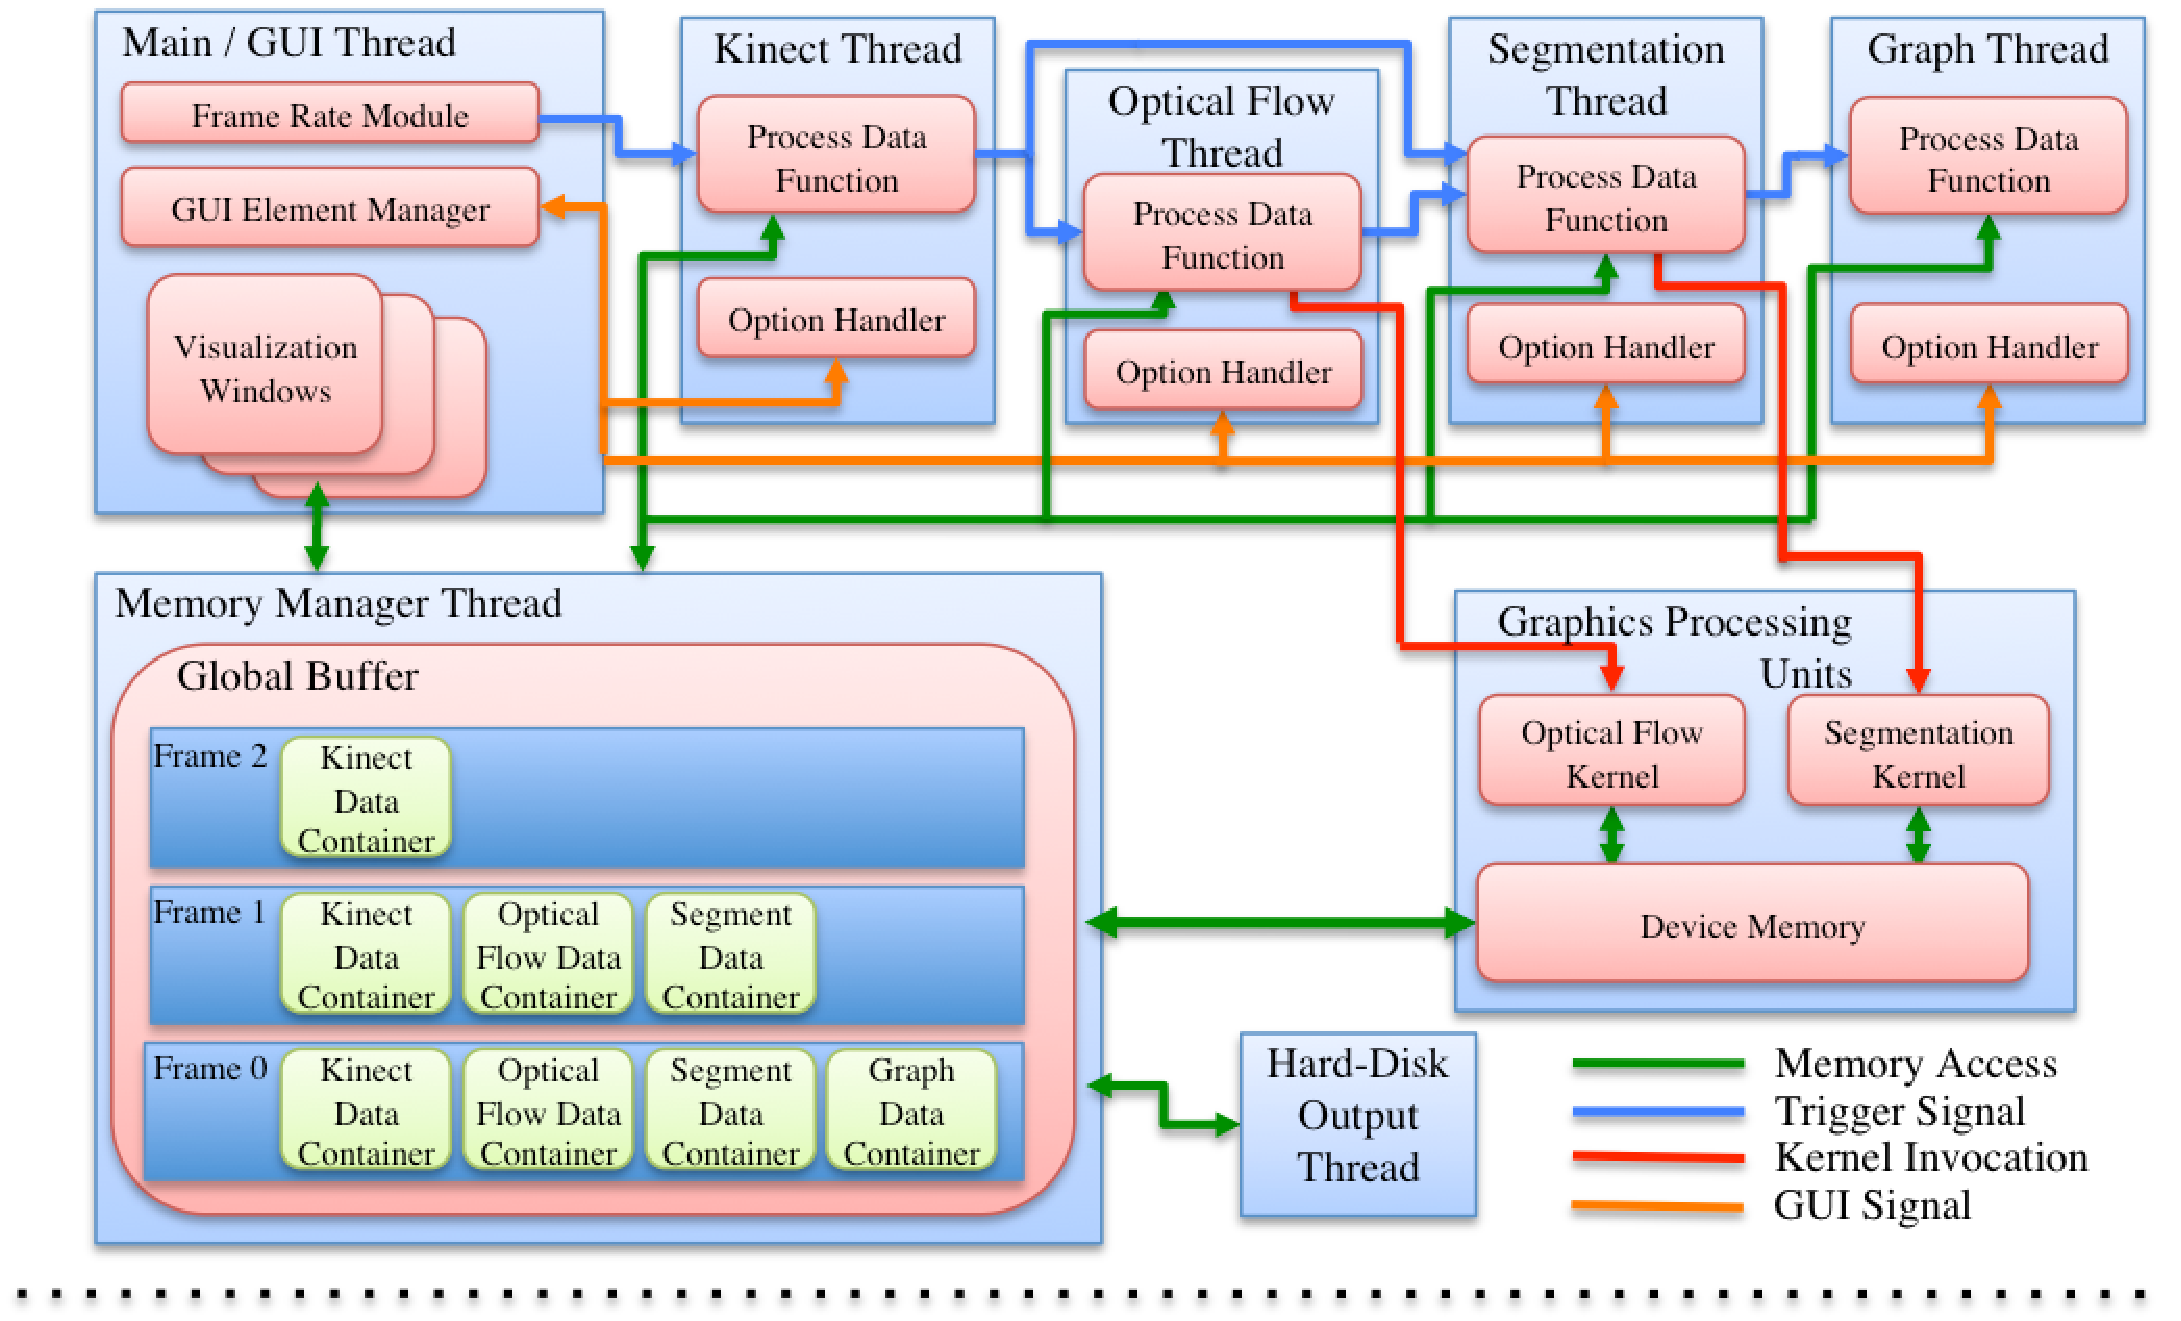
\includegraphics[width=165mm,height=100mm]{SystemFlowColor.pdf}
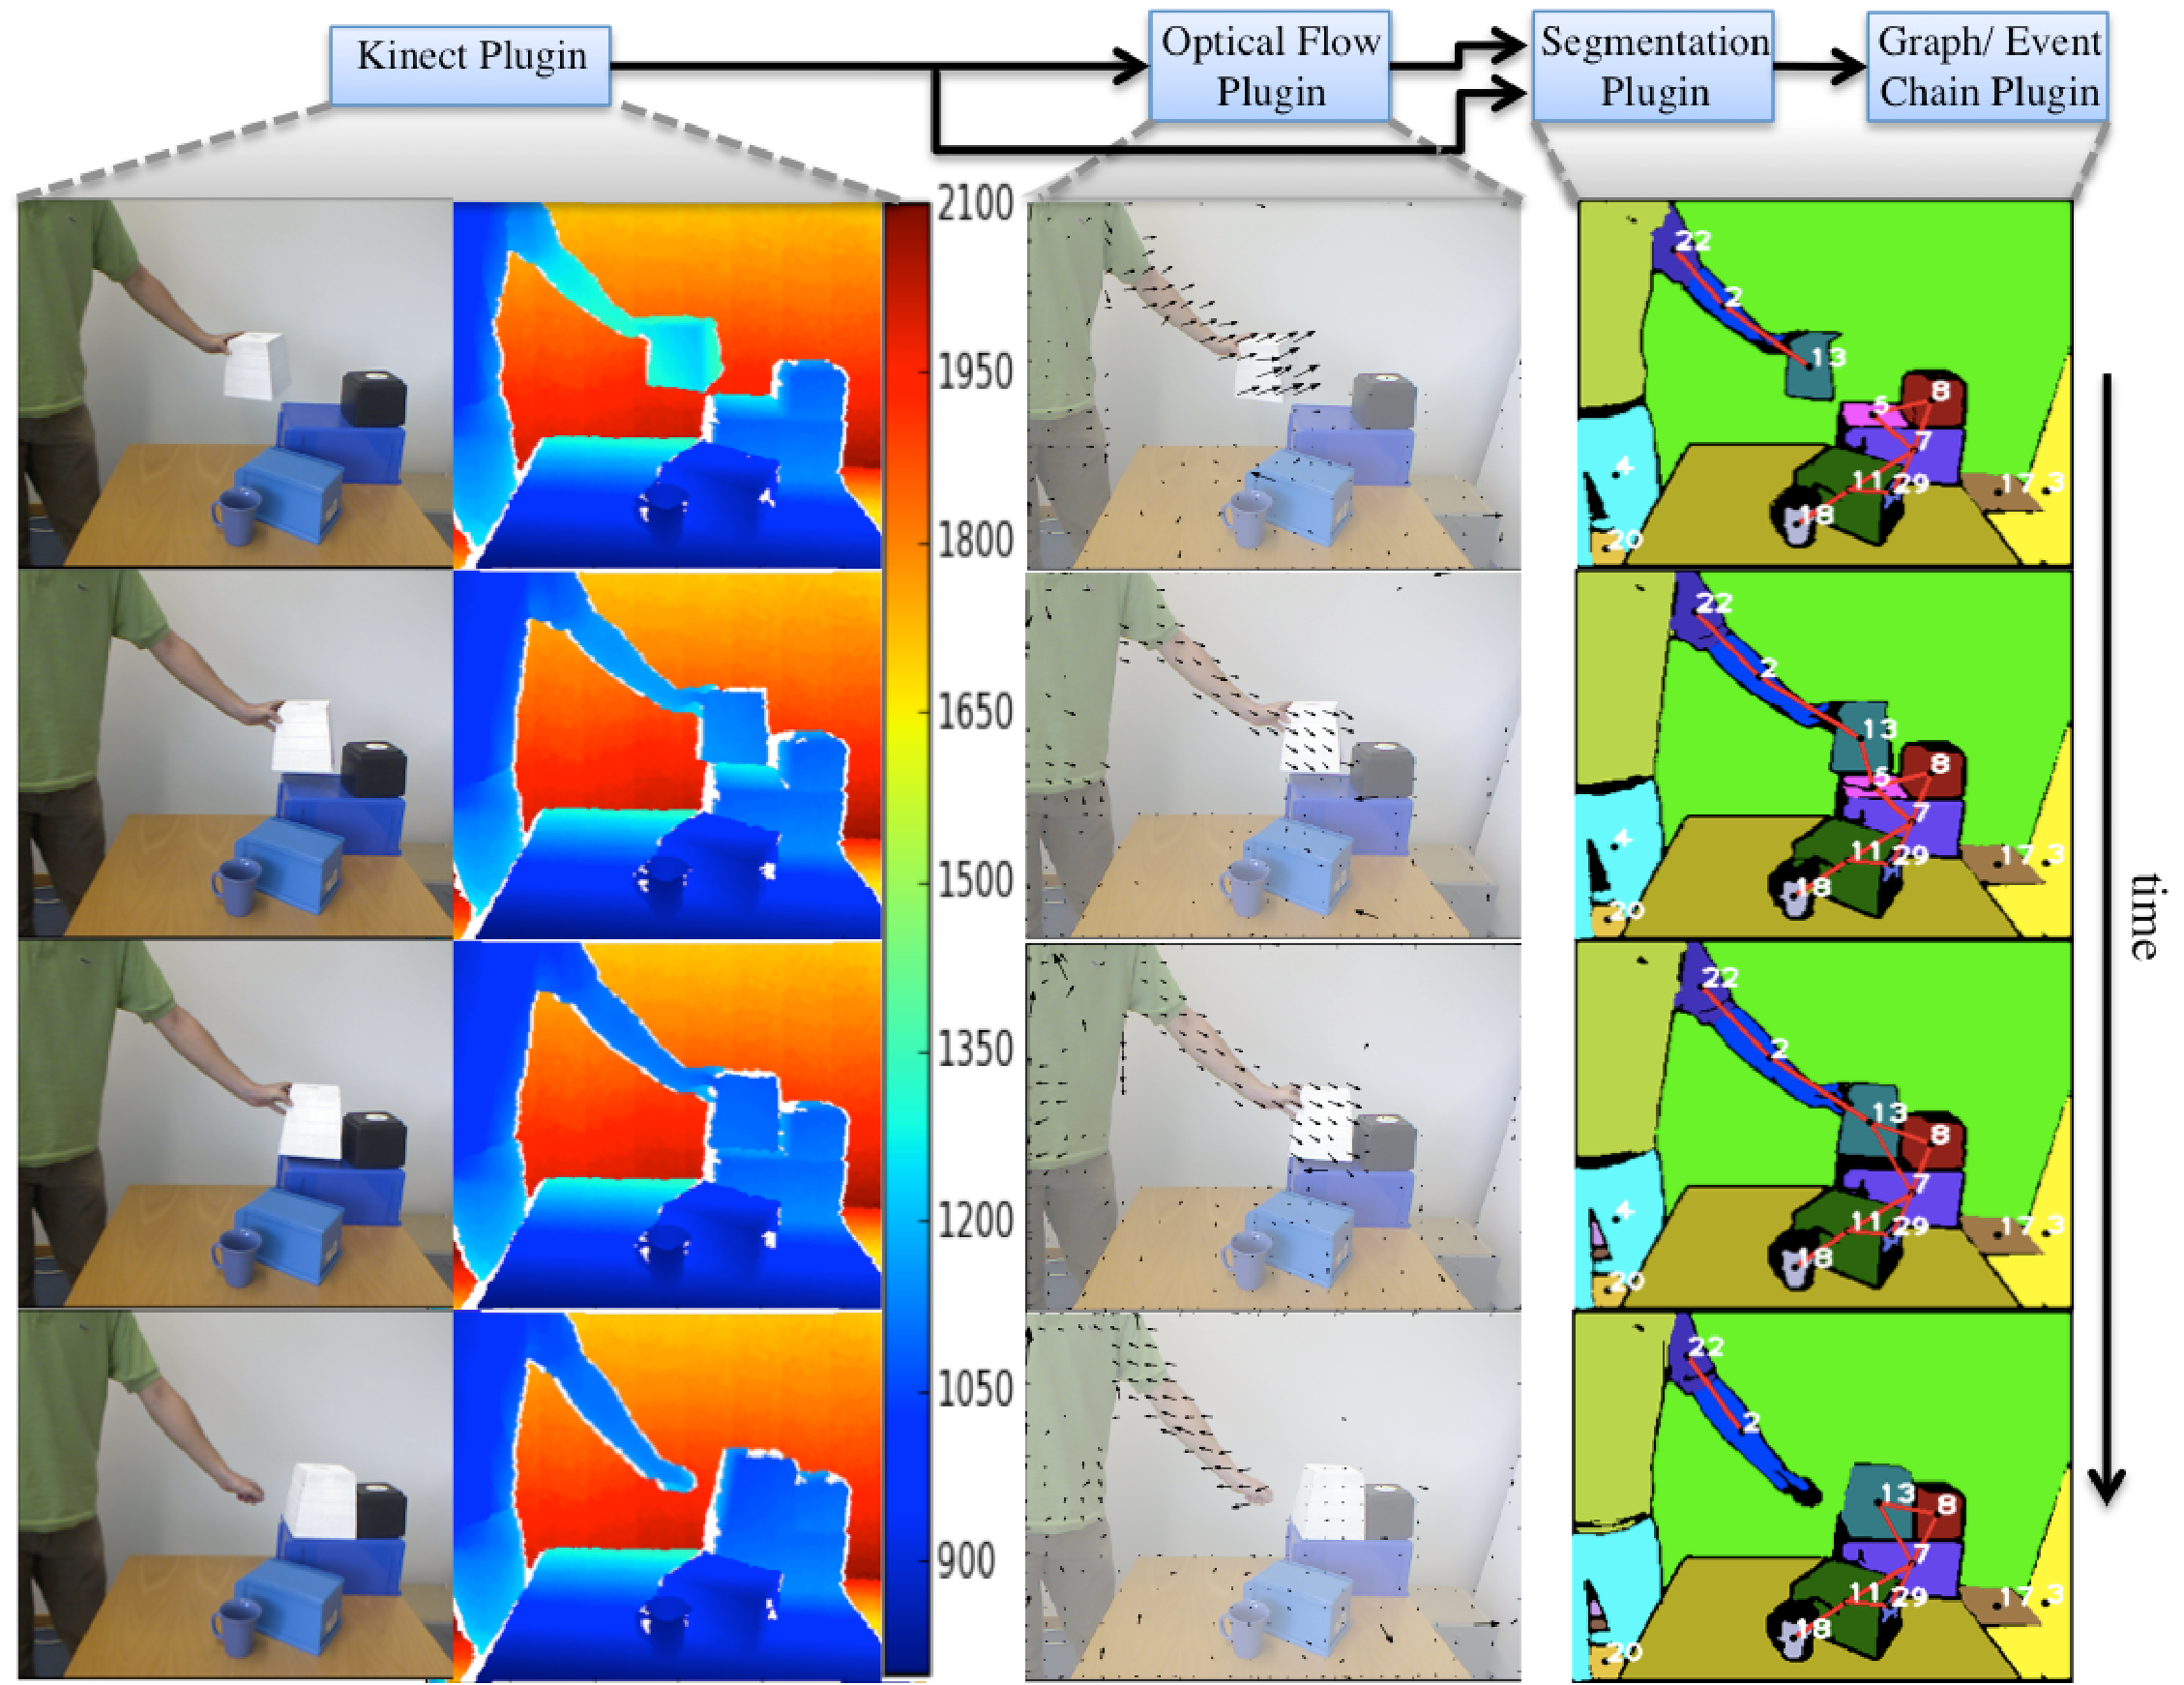
\includegraphics[width=170mm,height=112mm]{SystemOutput.pdf}
\end{center}
  \caption{Overview of the system architecture and demonstration system output for four frames. The colums show output from the different components; from left to right, Kinect image and depth (in mm), optical flow, and graphs overlaid on segmentation plugin output. This type of output can be seen live in any number of visualization windows within the GUI.}
\label{fig:SystemArchitecture}
\end{figure*}

\subsection{Plugin Development and Interaction}
The functionality of the system is provided primarily via plugins. A plugin consists of a shared library which is loaded dynamically at run-time. The system is based on the low-level Qt plugin API, which facilitates development and ensures compatibility across different platforms. Plugins inherit from a pure abstract interface class which defines a protocol for communicating with the core application. This permits plugins to define input and output types and pass messages to/from the GUI and memory manager. 

Developers are required to implement a \emph{processData} function, which receives input and writes to an output \emph{DataContainer}. The developer can optionally create any number of GUI elements (e.g. sliders, buttons) using the interface functions.  Plugins specify how many inputs they require, and give the possible types for these inputs. Communication between plugins is accomplished through a standardized data container interface. The core architecture contains commonly used data container implementations, such as \emph{StereoImageContainer}. Plugins may define their own specialized data containers which are loaded at runtime with the plugin. For example, the Segmentation plugin has its own container type \emph{SegmentationData}, which contains a list of labeled segments, metadata about the segments, and labeled images. The standardized data container interface allows for any plugin to refer to a new container class without actual knowledge of the container itself other then the string identifiers of 
its members (e.g. "Segment Labels"). Correct handling of access to these members is accomplished through dynamic dispatch using the virtual lookup table. This ensures that a plugin written by one researcher can be easily used as input to another's, as long as they know the proper identifiers and underlying formatting of the data. 


\subsection{Visualization}

During the development and use of a vision system, it is of utmost importance to be able to visualize what is occurring at every stage of the system pipeline. As such, our system allows users to create any number of visualization windows which can select any plugin to display (and which part of the plugin's output to display, e.g. left or right image). If a developer creates their own data container for a plugin, they can define a special visualization callback function as part of this container. The system will automatically detect this callback when the plugin is loaded, and use it for visualizing the plugin's output. Developers can specify multiple methods for visualizing the plugin; the GUI for visualization will allow selection of which to display.

Visualization windows read directly from the global buffer, and as such have a small memory overhead. Additionally, visualization runs in the GUI thread, rather than in any of the plugin threads. If a plugin slows down the system, visualization (and the GUI) will remain responsive, allowing the user to troubleshoot. This also means that visualization that requires computation, such as labeling an image with text or vector graphics, will have a negligible effect on the actual frame throughput of the system. If visualization lags behind the system output, frames are automatically skipped on an interval that allows visualization to maintain synchronization with the rest of the system. This is of particular importance in an online system, such as our real-time robotic application, where visualization lagging behind processing can cause confusion or even errors.

%%%%%%%%%%%%%%%%%%%%%%%%%%%%%%%%%%%%%%%%%%%%%%%%%%%%%%%%%%%%%%%%%%%%%%
%%%%%% MEMORY ARCHITECTURE %%%%%%%%%%%%%%%%
%%%%%%%%%%%%%%%%%%%%%%%%%%%%%%%%%%%%%%%%%%%%%%%%%%%%%%%%%%%%%%%%%%%%%%

\section{Memory Architecture}
The memory management system has been designed to allow distributed development and computing, complex system pipelines incorporating feedback loops, and efficient use of the GPU as a computational resource. The following subsections will describe how these design goals have been achieved by illustrating our \emph{Global Buffer} design and explaining how it manages GPU memory.  

\subsection{Global Buffer}
Our global buffer concept was designed to overcome the limitations of standard online vision pipelines. In a standard online pipeline a local buffering scheme is used; each algorithm has an input buffer, where data accumulates while it is waiting to be processed. Such a setup is adequate as long as the  pipeline remains unidirectional, but complications arise in using feedback loops.
\begin{figure}[t]
\begin{center}
   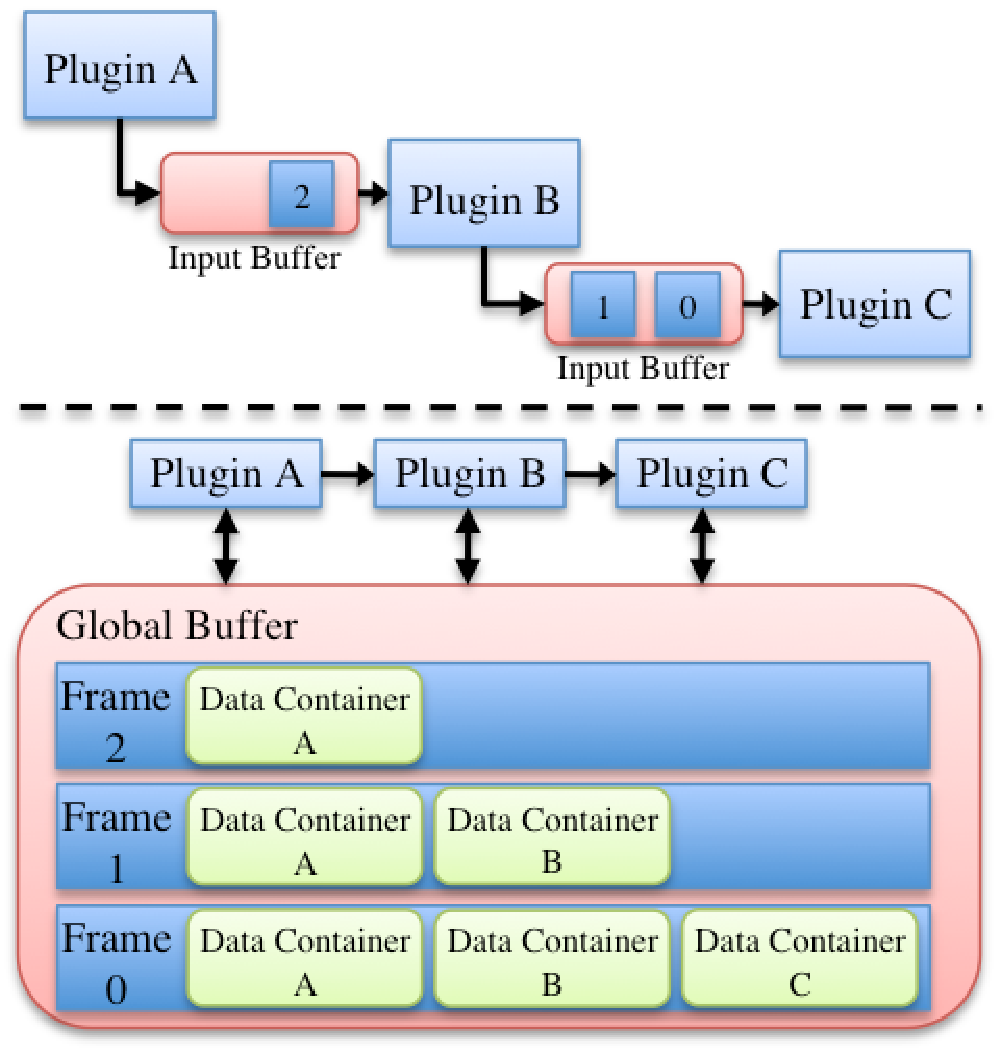
\includegraphics[width=0.6\linewidth]{BufferComparaison.pdf}
\end{center}
   \caption{A typical buffering scheme (top) and our buffer (bottom).}
\label{fig:BufferFig}
\end{figure}
Figure~\ref{fig:BufferFig} compares a standard pipeline with our global buffer; unlike a typical buffering scheme, our global buffer maintains and manages all memory in a central location (and separate thread). The global buffer is responsible for dynamic allocation of all data containers, maintaining reference counts, and determining when a frame can expire. Since the global buffer is responsible for maintaining memory, plugins use a message passing system to communicate. Plugins pass messages to each other to notify completion of a new frame, or to trigger a feedback mechanism. They also use the message passing system to request that the global buffer allocate a new data container for their output. When a developer creates a new type of data container, they use a simple interface to pass the global buffer a function pointer for creating an instance of their new data container type. 

In order to fully understand the limitations of a standard buffering system, consider, for instance, the system shown at the top of Figure~\ref{fig:Feedback}.  If the feedback mechanism is triggered for frame \emph{n}, plugin \emph{B} must return to frame \emph{n} in order to modify how it was processed. This is not possible in the standard local buffer scheme, as that data was discarded after it was used as input to \emph{B}. One possible solution is to maintain another local buffer for each plugin which contains data which has already been processed, but this quickly adds several degrees of complexity. In particular, garbage collection becomes very difficult, and management of these buffers when feedback does occur becomes unnecessarily convoluted.

\begin{figure}[t]
\begin{center}
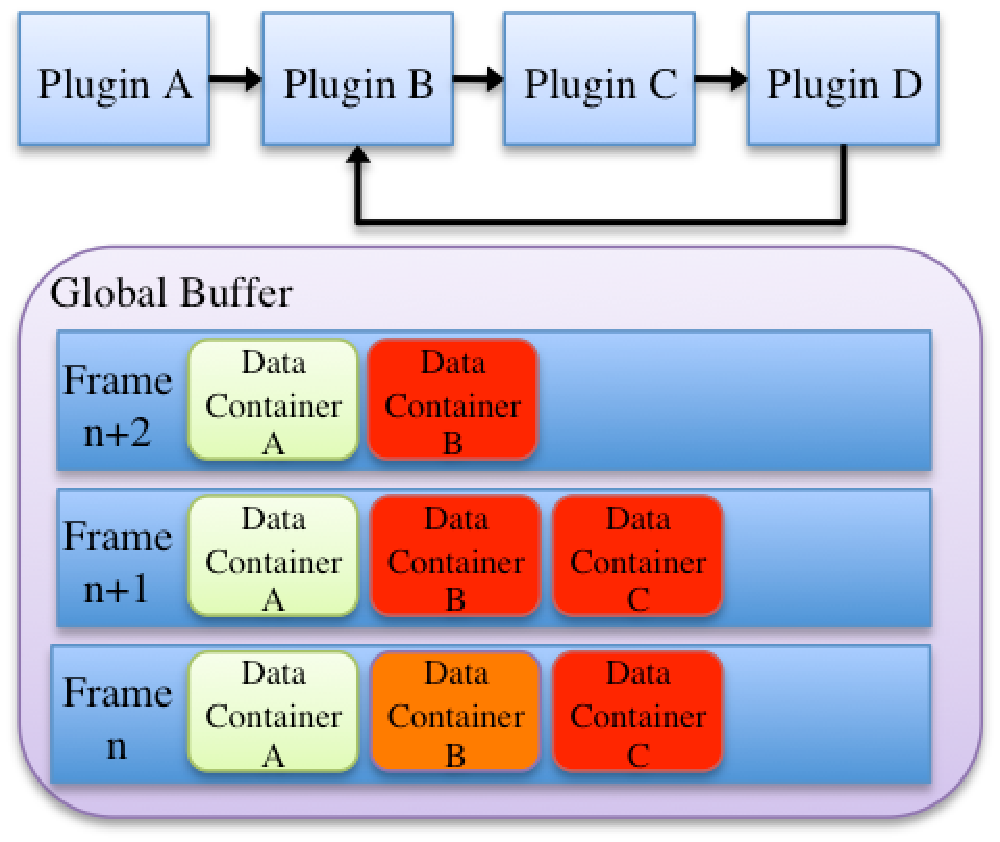
\includegraphics[width=0.6\linewidth]{Feedback.pdf}
\end{center}
   \caption{Feedback using a global buffer}
\label{fig:Feedback}
\end{figure}

The global buffer solves this by maintaining data in a more structured way. When a feedback mechanism is triggered for frame \emph{n} the triggering plugin (\emph{D}) sends a message to \emph{B}, causing it to stop processing what it has scheduled, and revert to frame \emph{n}. As frame \emph{n} is still easily accessible in the global buffer, \emph{B} can simply send a request for the pointer(s) to the input data container(s) it requires. The global buffer is guaranteed to still have the data for frame \emph{n}, because \emph{D} never produced an output for frame \emph{n}, so the global buffer has not marked frame \emph{n} as complete. Once \emph{B} finishes processing frame \emph{n} with its new feedback information, it will overwrite its old output for frame \emph{n} (shown in orange) and then simply continue on as it would normally, processing frame \emph{n+1}. The feedback corrected data will propagate down the pipeline, and any data which is no longer valid (shown in red) will simply be overwritten. 
Infinite feedback loops are avoided by a preventing feedback from occurring more than once per plugin per frame.

\subsection{GPU Memory Handling}
While utilizing the massively-parallel GPU as a coprocessor has become increasingly common, how to integrate it effectively into an open vision architecture remains an open question. Particularly vexing is how to integrate it seamlessly into the memory system of such an architecture, as the GPU has separate physical memory, which is entirely distinct in both location and structure from that used by the CPU \cite{NVIDIA_Fermi}. Data streaming through the system must be transferred to the GPU for modules which use it, and then transferred back out for visualization and used by modules later in the pipeline.

A naive implementation of this architecture would simply serialize the operations; when a module needs to use the GPU, it copies data to device memory, executes a kernel, and then copies the output back out to host memory. While this is still relatively efficient, it fails to fully take advantage of the pipelined streaming architecture, since the memory transfer bandwidth is idle while the kernel is executing. The architecture uses the streaming CUDA API to utilize this spare bandwidth, allowing it to perform concurrent asynchronous memory transfer and kernel execution. 

\begin{figure}[t]
\begin{center}
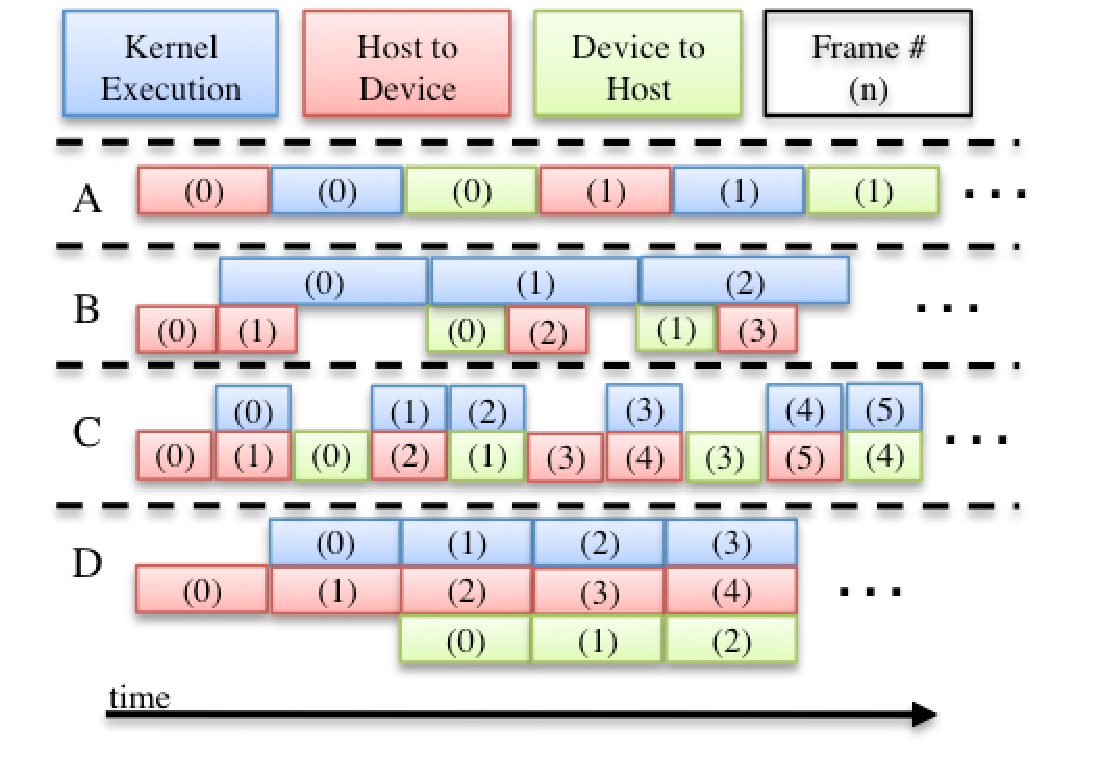
\includegraphics[width=0.7\linewidth]{ConcurrentGPU.pdf}
\end{center}
   \caption{Streaming; Concurrent kernel execution}
\label{fig:Streaming}
\end{figure}

As shown in Figure~\ref{fig:Streaming}, we utilize a pre-caching technique, whereby data for frame~\emph{n+1} is transferred during the execution of frame~\emph{n}. When the kernel execution time is significantly longer than the transfer time (\emph{B}), memory transfer is completely hidden, even with unidirectional memory. When kernel execution time is comparable to memory transfer time, only some of the transfer can be hidden (\emph{C}), unless the hardware supports concurrent data transfers\footnote{Concurrent data transfers are supported under the Fermi architecture\cite{NVIDIA_Fermi}. Currently the Fermi Quadro and Tesla series cards have two Direct memory access (DMA) engines\cite{NVIDIA_Concurrent}, allowing them to perform host-to-device and device-to-host operations simultaneously. The consumer Fermi cards (GTX 4xx, 5xx) only have a single DMA engine, so concurrent transfers are disabled on them.}  (\emph{D}).


%%%%%%%%%%%%%%%%%%%%%%%%%%%%%%%%%%%%%%%%%%%%%%%%%%%%%%%%%%%%%%%%%%%%%%
%%%%%% DEMO SYSTEM %%%%%%%%%%%%%%%%
%%%%%%%%%%%%%%%%%%%%%%%%%%%%%%%%%%%%%%%%%%%%%%%%%%%%%%%%%%%%%%%%%%%%%%

\section{Demonstration System}
This section presents a real-time demonstration system, consisting of six plugins. The demonstration system calculates dense disparity using a standard stereo camera setup (rather than Kinect data) in order to show the flexibility of the architecture as well as highlight the speedup achieved via multithreading. Switching from Kinect input to a stereo camera setup is simply a matter of changing connections in the GUI. The pipeline described consists of plugins for reading  and rectifying stereo data, calculating optical flow\cite{PauwelsArchitecture}, computing disparity\cite{PauwelsArchitecture}, segmentation and tracking\cite{Abramov_3DSegmentation}, dense disparity estimation, and semantic graph and event chain generation\cite{Aksoy10,Aksoy11}. This type of a system configuration is used to recognize and learn object manipulation actions in a robotics context.

\subsection{Image Acquisition}
Video is acquired using a Firewire stereo camera rig. Triggering for image acquisition can be controlled using either an external hardware trigger or the architecture's software clock. Rectification is performed on the GPU (there is a separate plugin for calibration using a standard chessboard). Time from triggering to output of a rectified pair of stereo images is around 10ms at 1024x768.
%Support for the Microsoft Kinect camera is provided via the OpenNI library \cite{openNI}, along with the NITE middleware \cite{NITE}. The Kinect is an especially attractive option as an input source, as it provides both images and high quality disparity maps synchronized at 30fps. Raw Kinect disparity is transformed to a normalized depth, and then rectified to align with the video stream~\cite{Burrus_KinectCal}.  

\subsection{Disparity and Optical Flow}
Optical flow is computed using the GPU implementation \cite{PauwelsArchitecture} of a phase-based algorithm \cite{Gautama_OpticalFlow}. The algorithm tracks the temporal evolution of equi-phase contours by taking advantage of phase constancy. Differentiation of the equi-phase contours with respect to time yields spatial and temporal phase gradients. Optical flow is then computed by integrating the temporal phase across orientation. Estimates are refined by traversing a Gabor pyramid from coarser to fine levels. The plugin uses the five most recent frames to compute optical flow in the case of online video, but can also use "future" frames when working with recorded movies (this can slightly improve the quality of output flow). 

Sparse disparity maps are computed on the GPU using a technique similar to optical flow \cite{PauwelsArchitecture}. Rather than use temporal phase gradients, the disparity algorithm relies on phase differences between stereo-pair rectified images. As with the optical flow algorithm, results are computed using a coarse to fine pyramid scheme. 

\subsection{Segmentation and Tracking}
The segmentation and segment tracking plugin has two roles; first, it partitions the image into labeled regions, as seen in the right-most column of Figure~\ref{fig:SystemArchitecture}, and second, it determines correspondences between frames to maintain consistent labeling. The segmentation algorithm is based on the work of Blatt et al. \cite{Blatt_SuperClustering}, which applies the Potts model in such a way that superparamagnetic phase regions of aligned spins correspond to a natural partition of the image data. Initial spins are assigned to pixels randomly, and then a Metropolis-Hastings algorithm with annealing \cite{Abramov_3DSegmentation} is used to iteratively update the spins until an equilibrium state is reached. 

The Metropolis algorithm is implemented on the GPU\cite{Abramov_3DSegmentation}, permitting real-time performance. The algorithm itself lends itself to efficient implementation on a GPU, as interactions are only computed locally (8 connected nearest-neighbors). Coupling interactions between pixels are determined using average color vector difference (in the HSV space) of nearest-neighbors. Additionally, when depth data is available, the algorithm prevents interactions between pixels if there is a significant difference in their depth values. This prevents coupling across regions which have similar color but discontinuous depth. 

In addition to segmentation, the plugin maintains consistent labels for objects from frame to frame. This is accomplished by transferring spins between frames using output from an optical-flow plugin \cite{Abramov_3DSegmentation}. As such, only the first frame is actually initialized at random; subsequent frames are initialized using a forward-propagated version of the previous frame's equilibrium spins. This has two advantages; the number of iterations needed to reach equilibrium is greatly reduced since the spin distribution already approximates the final state, and the algorithm naturally tracks objects since spins (and thus labels) are maintained over time.
 
\subsection{Semantic Graphs}
The semantic graphs plugin constructs a symbolic 3D description of the scene from the segmentation results and disparity maps. Segments are used to construct undirected and un-weighted graphs (seen in the right-most column of Figure~\ref{fig:SystemArchitecture}; nodes are labeled with numbers and red lines are graph edges). Each segment is given a node and edges represent their three dimensional touching relations. Graphs can change by continuous distortions (lengthening or shortening of edges) or, more importantly, through discontinuous changes (nodes or edges can appear or disappear). Such a discontinuous change represents a natural breaking point: All graphs before are topologically identical and so are those after the breaking point. Hence, we can apply an exact graph-matching method \cite{Sumsi08} at each breaking point and extract the corresponding topological main graphs. The sequence of these main graphs thus represents all structural changes (manipulation primitives) in the scene. 

This type of graph representation is then encoded by a semantic event chain (SEC), which is a sequence-table; rows and columns of which represent possible spatial relations between each segment pair and manipulation primitive. This final output can be used to classify manipulations and categorize manipulated objects for use in a robotics or human-computer interaction (HCI) setting\cite{Aksoy10,Aksoy11}. The primary advantage of this method is that actions can be analyzed without models or a-priori representation; the dynamics of an action can be acquired without needing to know the identities of the objects involved.

\begin{figure*}[t]
\begin{center}
   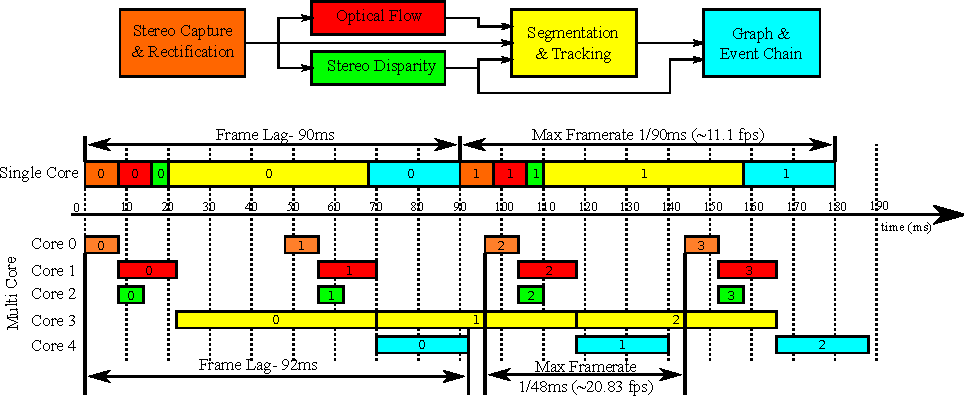
\includegraphics[width=0.98\linewidth,height=65mm]{TimingResults.pdf}
\end{center}
   \caption{Timing results for demonstration system; plugins are color coded and contain frame numbers. When run in single thread mode, short GPU operations such as optical flow are significantly faster due to reduced overhead; this results in slightly lower (2ms) frame lag. The true benefit of multi-threaded mode is the higher maximum frame-rate that can be achieved. }
\label{fig:TestMTST}
\end{figure*}



%%%%%%%%%%%%%%%%%%%%%%%%%%%%%%%%%%%%%%%%%%%%%%%%%%%%%%%%%%%%%%%%%%%%%%
%%%%%% PERFORMANCE %%%%%%%%%%%%%%%%
%%%%%%%%%%%%%%%%%%%%%%%%%%%%%%%%%%%%%%%%%%%%%%%%%%%%%%%%%%%%%%%%%%%%%%

\section{Results and Discussion}

Testing was performed to compare single threaded with multi-threaded operation mode and to detect the impact of visualization on processing speed. Testing was performed on an Intel i7 (3.33Ghz, 8 execution threads) system with an NVIDIA GTX 295 GPU. The demonstration setup depicted at the top of Figure~\ref{fig:TestMTST} was used for all tests. To determine if visualization had a negative impact, the tests were run with and without a visualization windows for each component, showing live views of their outputs. Timing measurements for plugins are the mean execution time per frame of a 1000 frame (640x480) stereo video sequence (frames of which are shown in Figure~\ref{fig:SystemArchitecture}), averaged over 10 runs. The code for the single and multi-threaded versions is identical with the exception of the movement of plugin objects to separate threads.

We measure performance by analyzing two key attributes of a pipelined vision real-time vision system. First, in terms of frame lag, that is time from frame acquisition to final output, multi-threaded mode is slightly slower than single-threaded. As shown in Figure~\ref{fig:TestMTST}, this is due to relatively fast plugins which use the GPU (disparity and optical flow in this case). This can be attributed to the static overhead cost incurred by switching between threads while using the CUDA run-time API. The switching is relatively expensive for short GPU operations as it forces the CUDA driver to create and destroy GPU contexts\footnote{GPU contexts are analogous to CPU processes, and each have their own distinct address space. Each thread may only have one context active at a time, and contexts may not share threads. See \cite{NVIDIA_Fermi, NVIDIA_CUDA} for more details.}. This could be avoided by the addition of an additional GPU; in our demonstration system the driver is forced to change contexts as there 
are three threads (flow, disparity, segmentation) attempting to use two GPUs. Additionally, the architecture will soon be brought to the newest CUDA release, which allows context sharing between threads. It should also be noted that at higher resolutions multi-threaded mode overtakes single-threaded, as the overhead cost of context switching is outweighed by the gain from computing optical flow and disparity in parallel. 

The second measure of performance, throughput, or maximum frame rate, shows a significant speedup in multi-threaded mode, almost doubling from 11.1 (stereo)fps to 20.83. While significant, the speedup is not equal to the number of execution threads used by the demonstration setup (six; one for each plugin and one for the GUI \& memory manager). This less-than-optimal gain can be attributed to the fact that the demonstration system had one component, segmentation \& tracking, which was significantly slower then the rest. As seen in Figure~\ref{fig:TestMTST}, the entire system throughput is limited by the rate at which the segmentation plugin produces output. 

As seen in Figure~\ref{fig:TestVis}, the addition of visualization components has a small impact on performance. This delay was most noticeable for the shorter components, disparity and optical flow, but never exceeded 2ms. Fortunately, this additional time does not affect throughput in multi-threaded mode, as it is hidden by the length of the longest component. The times with visualization were used for Figure~\ref{fig:TestMTST}; clearly shortening the time of any component other than segmentation will have a negligible effect on performance. While the increase does not affect throughput, it has a slight effect on frame lag. Frame lag is less important than throughput for our research, but it should be noted that in certain cases, such as when quick reactions are required, frame lag may be an important performance measure. 

\begin{figure}[t]
\begin{center}
   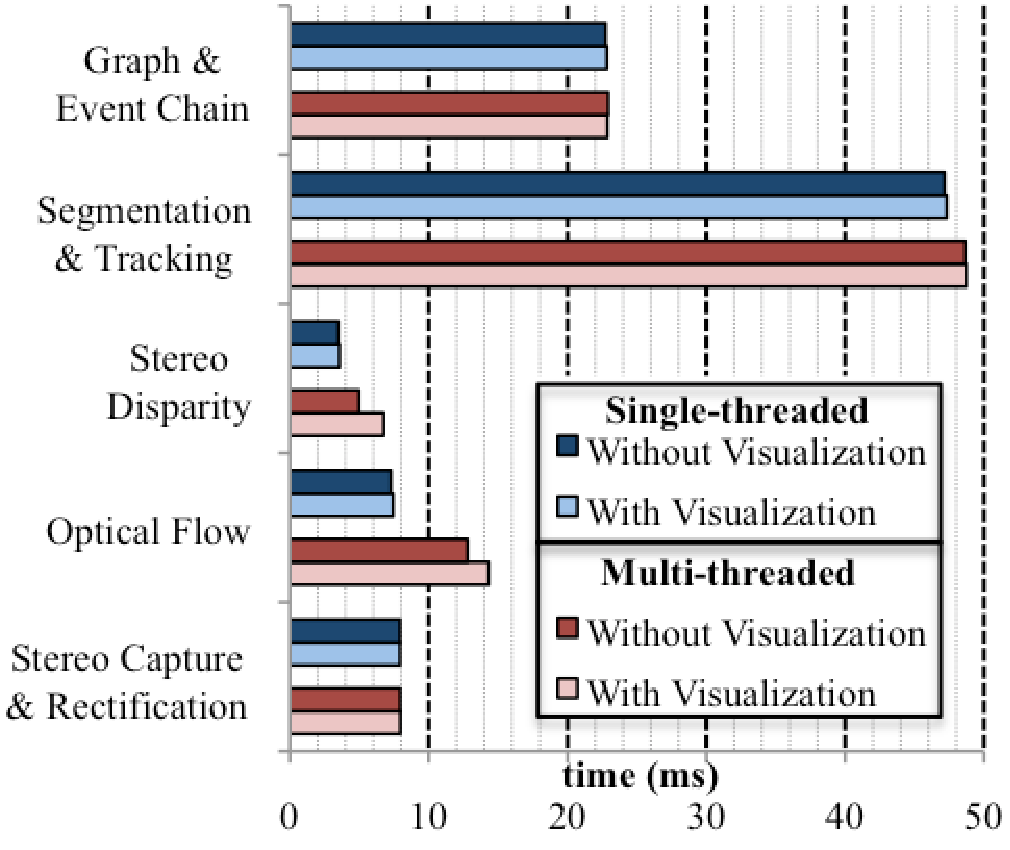
\includegraphics[width=0.5\linewidth]{TimingGraph.pdf}
\end{center}
   \caption{Visualization has a slight impact on performance, but the effect is negligible in multi-threaded mode where the slight increases in processing time are hidden in the length of the longest component (in this case, segmentation).}
\label{fig:TestVis}
\end{figure}


%%%%%%%%%%%%%%%%%%%%%%%%%%%%%%%%%%%%%%%%%%%%%%%%%%%%%%%%%%%%%%%%%%%%%%
%%%%%% CONCLUSION %%%%%%%%%%%%%%%%
%%%%%%%%%%%%%%%%%%%%%%%%%%%%%%%%%%%%%%%%%%%%%%%%%%%%%%%%%%%%%%%%%%%%%%
\section{Conclusion}
Building a self-contained, efficient, and complete vision system acts as a significant barrier to entry for those wishing to develop and test new vision algorithms. We have presented a modular plugin environment, designed specifically for expandability and parallel architectures, which facilitates rapid distributed development of vision pipelines. Our plugin system allows simple collaboration between organizations, allowing developers to share algorithms easily, and without forcing them to share code. The architecture permits streaming use of the GPU as a coprocessor, efficient visualization of algorithm outputs, and the ability to use complex pipelines involving feedback mechanisms. The system architecture has been released released under an open-source GPL license\footnote{\url{https://launchpad.net/oculus}}.